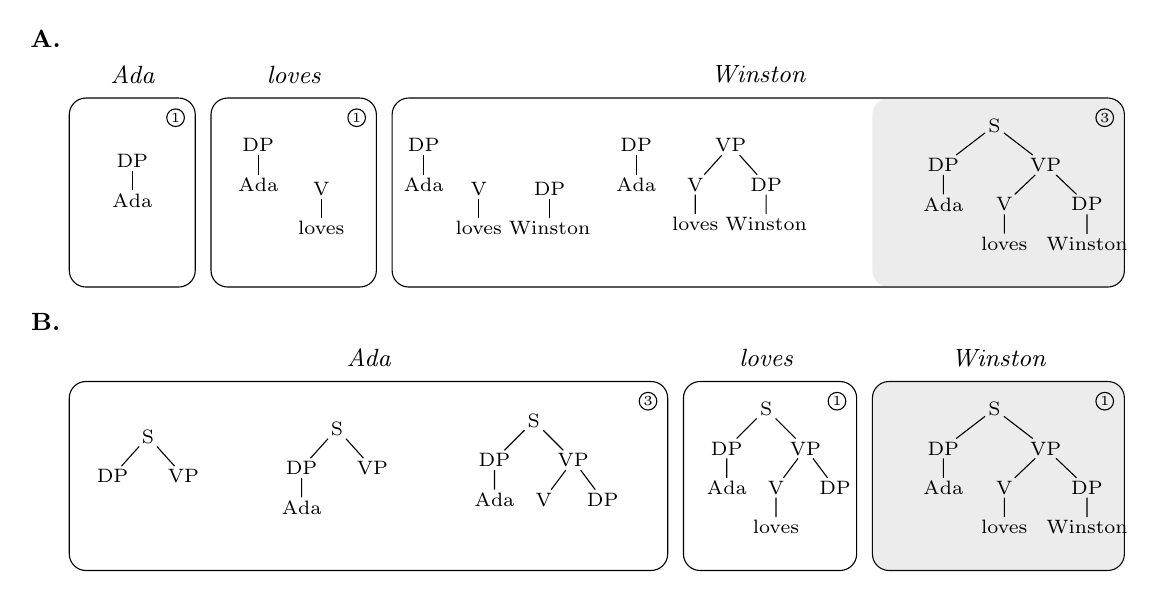
\begin{tikzpicture}[every node/.style={font=\scriptsize, inner sep=1pt},
  level distance=0.5cm,
  level 1/.style={sibling distance=0.9cm},
  level 2/.style={sibling distance=0.75cm},
  num/.style={circle, draw, inner sep=0.6pt, font=\tiny},
  hd/.style={font=\small\itshape}]
% ---------------- Panel A: bottom-up ----------------
\node[font=\small\bfseries] at (-0.3,0.75) {A.};
\draw[rounded corners=6pt] (0,-2.4) rectangle (1.6,0);
\draw[rounded corners=6pt] (1.8,-2.4) rectangle (3.9,0);
\draw[rounded corners=6pt] (4.1,-2.4) rectangle (13.4,0);
\fill[gray, fill opacity=0.15, rounded corners=6pt] (10.2,-2.4) rectangle (13.4,0);
\node[hd] at (0.8,0.3) {Ada};
\node[hd] at (2.85,0.3) {loves};
\node[hd] at (8.75,0.3) {Winston};
\node[num] at (1.35,-0.25) {1};
\node[num] at (3.65,-0.25) {1};
\node[num] at (13.15,-0.25) {3};
% box 1
\node at (0.8,-0.8) {DP} child {node {Ada}};
% box 2
\node at (2.4,-0.6) {DP} child {node {Ada}};
\node at (3.2,-1.15) {V} child {node {loves}};
% box 3
\node at (4.5,-0.6) {DP} child {node {Ada}};
\node at (5.2,-1.15) {V} child {node {loves}};
\node at (6.1,-1.15) {DP} child {node {Winston}};
\node at (7.2,-0.6) {DP} child {node {Ada}};
\node at (8.4,-0.6) {VP}
  child {node {V} child {node {loves}}}
  child {node {DP} child {node {Winston}}};
\node at (11.75,-0.35) {S}
  child[sibling distance=1.3cm] {node {DP} child {node {Ada}}}
  child[sibling distance=1.3cm] {node {VP}
    child[sibling distance=1.05cm] {node {V} child {node {loves}}}
    child[sibling distance=1.05cm] {node {DP} child {node {Winston}}}};
% ---------------- Panel B: top-down ----------------
\begin{scope}[yshift=-3.6cm]
\node[font=\small\bfseries] at (-0.3,0.75) {B.};
\draw[rounded corners=6pt] (0,-2.4) rectangle (7.6,0);
\draw[rounded corners=6pt] (7.8,-2.4) rectangle (10.0,0);
\draw[rounded corners=6pt] (10.2,-2.4) rectangle (13.4,0);
\fill[gray, fill opacity=0.15, rounded corners=6pt] (10.2,-2.4) rectangle (13.4,0);
\node[hd] at (3.8,0.3) {Ada};
\node[hd] at (8.85,0.3) {loves};
\node[hd] at (11.8,0.3) {Winston};
\node[num] at (7.35,-0.25) {3};
\node[num] at (9.75,-0.25) {1};
\node[num] at (13.15,-0.25) {1};
\node at (1.0,-0.7) {S} child {node {DP}} child {node {VP}};
\node at (3.4,-0.6) {S} child {node {DP} child {node {Ada}}} child {node {VP}};
\node at (5.9,-0.5) {S}
  child[sibling distance=1.0cm] {node {DP} child {node {Ada}}}
  child[sibling distance=1.0cm] {node {VP} child {node {V}} child {node {DP}}};
\node at (8.85,-0.35) {S}
  child[sibling distance=1.0cm] {node {DP} child {node {Ada}}}
  child[sibling distance=1.0cm] {node {VP} child {node {V} child {node {loves}}} child {node {DP}}};
\node at (11.75,-0.35) {S}
  child[sibling distance=1.3cm] {node {DP} child {node {Ada}}}
  child[sibling distance=1.3cm] {node {VP}
    child[sibling distance=1.05cm] {node {V} child {node {loves}}}
    child[sibling distance=1.05cm] {node {DP} child {node {Winston}}}};
\end{scope}
\end{tikzpicture}
